% ============================================
% AEGIS Entropy — Final Report
% Adaptive Entropy-based Gateway for Intrusion Suppression
% ENSA Kénitra — RST S6 — Module: Intelligence Artificielle
% June 2026
% Structure conforme au sommaire exigé par le professeur
% ============================================
\documentclass[12pt,a4paper]{report}

% --- Encoding & Language ---
\usepackage[utf8]{inputenc}
\usepackage[T1]{fontenc}
\usepackage[english]{babel}
\usepackage{lmodern}

% --- Page Layout ---
\usepackage[left=2.5cm,right=2.5cm,top=2.5cm,bottom=2.5cm]{geometry}
\setlength{\parindent}{0pt}
\setlength{\parskip}{0.65em}
\renewcommand{\arraystretch}{1.25}

% --- Math ---
\usepackage{amsmath,amssymb}

% --- Graphics ---
\usepackage{graphicx}
\graphicspath{
    {figures/}
    {figures/data/}
    {figures/capture/}
}
\usepackage{float}
\usepackage{caption}
\usepackage{subcaption}

% --- Tables ---
\usepackage{array}
\usepackage{longtable}
\usepackage{booktabs}
\usepackage{tabularx}
\usepackage[table]{xcolor}

% --- Lists ---
\usepackage{enumitem}
\setlist[itemize]{topsep=0.2em,itemsep=0.2em}
\setlist[enumerate]{topsep=0.2em,itemsep=0.25em}

% --- Code Listings ---
\usepackage{listings}
\lstdefinestyle{pythonstyle}{
    language=Python,
    basicstyle=\ttfamily\small,
    keywordstyle=\color{blue}\bfseries,
    stringstyle=\color{red},
    commentstyle=\color{gray}\itshape,
    numbers=left,
    numberstyle=\tiny\color{gray},
    stepnumber=1,
    numbersep=5pt,
    backgroundcolor=\color{gray!5},
    frame=single,
    rulecolor=\color{gray!30},
    breaklines=true,
    showstringspaces=false,
    tabsize=4,
    captionpos=b
}
\lstset{style=pythonstyle}

% --- TikZ ---
\usepackage{tikz}
\usetikzlibrary{shapes.geometric, arrows.meta, positioning, calc, decorations.pathmorphing, fit, backgrounds}
\usepackage{pgfplots}
\pgfplotsset{compat=1.18}

% --- Colors for diagrams ---
\definecolor{darkbg}{HTML}{0b0f19}
\definecolor{cyan}{HTML}{22d3ee}
\definecolor{green}{HTML}{34d399}
\definecolor{red}{HTML}{f87171}
\definecolor{amber}{HTML}{fbbf24}
\definecolor{purple}{HTML}{a78bfa}
\definecolor{codebg}{HTML}{1a2332}
\definecolor{codegray}{HTML}{94a3b8}
\definecolor{LightGray}{HTML}{F2F2F2}
\definecolor{LightBlue}{HTML}{D9EAF7}

% --- Hyperlinks ---
\usepackage{hyperref}
\hypersetup{
    colorlinks=true,
    linkcolor=blue!70!black,
    urlcolor=blue!60!black,
    citecolor=blue!70!black,
    pdftitle={AEGIS Entropy --- Final Report},
    pdfauthor={AEGIS Entropy Team}
}

% --- Headers & Footers ---
\usepackage{fancyhdr}
\pagestyle{fancy}
\fancyhf{}
\fancyhead[L]{\small\textsc{AEGIS Entropy}}
\fancyhead[R]{\small\textsc{Final Report}}
\fancyfoot[C]{\thepage}
\renewcommand{\headrulewidth}{0.4pt}

% --- Chapter/Section Formatting ---
\usepackage{titlesec}
\titleformat{\chapter}[display]
    {\normalfont\Large\bfseries\color{blue!80!black}}
    {\chaptertitlename\ \thechapter}
    {0.5em}
    {}
\titleformat{\section}{\normalfont\large\bfseries\color{blue!70!black}}{\thesection}{1em}{}
\titleformat{\subsection}{\normalfont\normalsize\bfseries\color{blue!60!black}}{\thesubsection}{1em}{}

% --- Custom Commands ---
\newcolumntype{Y}{>{\raggedright\arraybackslash}X}
\newcolumntype{L}[1]{>{\raggedright\arraybackslash}p{#1}}
\newcommand{\code}[1]{\texttt{\detokenize{#1}}}

% --- Guillemets for French text ---
\usepackage[T1]{fontenc}
\newcommand{\og}{\guillemotleft\,}
\newcommand{\fg}{\,\guillemotright}

% ============================================
\begin{document}

% ============================================
% COVER PAGE
% ============================================
\begin{titlepage}
\centering

% --- Logos at top corners ---
\begin{minipage}{0.45\textwidth}

\includegraphics[width=2.5cm]{logo-UIT.png}
\end{minipage}%
\hfill
\begin{minipage}{0.45\textwidth}
\raggedleft

\includegraphics[width=2.5cm]{ensa_logo.png}
\end{minipage}

\vspace{1cm}

% --- Institution ---
{\Large\textsc{Universit\'{e} Ibn Tofa\"{i}l --- K\'{e}nitra}}\\[0.3cm]
{\large\textsc{\'{E}cole Nationale des Sciences Appliqu\'{e}es de K\'{e}nitra}}\\[0.3cm]
{\normalsize\textsc{Fili\`{e}re : Ing\'{e}nierie des R\'{e}seaux et des Syst\`{e}mes de T\'{e}l\'{e}communication}}

\vspace{2cm}

\rule{\textwidth}{0.5pt}\\[0.8cm]

{\Huge\bfseries AEGIS Entropy}\\[0.4cm]
{\Large Machine Learning-Based Intrusion Detection\\and Active Defense System}

\vspace{0.8cm}
\rule{\textwidth}{0.5pt}

\vspace{2cm}

% --- Supervisor + Team ---
\begin{minipage}{0.85\textwidth}
\centering
\textbf{Encadr\'{e} par}\\[0.3cm]
Prof.\ Aniss Moumen\\[1cm]
\textbf{R\'{e}alis\'{e} par}\\[0.3cm]
\begin{tabular}{c}
Adil Lekhbioui \\
Khadija Nafia \\
El Yazid Hammoubel \\
Moulay Anas \\
El Kartouti Anas \\
\end{tabular}
\end{minipage}

\vfill

{\normalsize Ann\'{e}e universitaire 2025 -- 2026}
\end{titlepage}

% ============================================
% TABLE OF CONTENTS
% ============================================
\tableofcontents
\clearpage

% ============================================
% 1. INTRODUCTION
% ============================================
\chapter{Introduction}

\section{Contexte et situation actuelle}

In the domain of network security, the early detection of reconnaissance activities constitutes a critical challenge. \textit{Port Scanning} --- the technique by which an attacker systematically probes a network's ports to identify active hosts, exposed services, and exploitable vulnerabilities --- represents the first phase of nearly all documented cyberattacks under the \textit{Cyber Kill Chain} model.

Currently, network infrastructures rely primarily on static rule-based firewalls and signature-based Intrusion Detection Systems (IDS) such as Snort and Suricata. These tools operate by recognizing known patterns and applying fixed thresholds. The shortcomings of this approach are well documented:

\begin{itemize}[nosep,leftmargin=1.5em]
  \item \textbf{Blindness to stealthy and slow scans:} attackers deliberately space their probes to stay below detection thresholds, rendering static rules ineffective.
  \item \textbf{High false positive rates:} legitimate traffic --- software updates, service discovery, monitoring tools --- frequently triggers the same signatures as malicious scans.
  \item \textbf{Absence of behavioral profiling:} current systems treat each packet in isolation, without analyzing temporal and statistical traffic patterns per source address over sliding time windows.
  \item \textbf{Inability to classify scan types:} a classic IDS does not distinguish a \textit{SYN Stealth Scan} from a \textit{UDP Scan}, depriving the analyst of essential tactical information.
\end{itemize}

These limitations directly impact SOC teams in terms of reaction time, alert reliability, and the ability to contain an attack before it progresses to more destructive phases. The continuous digitalisation of organisations has turned network infrastructures into critical assets shared across LAN, cloud, wireless, and hybrid environments. Protecting these infrastructures is no longer limited to deploying firewalls or signature-based systems; attackers now operate with adaptive, automated tools.

\section{Problem Statement}

The core problem is therefore twofold: port scanning and network reconnaissance are the precursors of most targeted attacks, yet current defences are either too slow to react, too rigid to detect novel techniques, or unable to respond autonomously. In this context, several fundamental questions arise:

\begin{enumerate}[nosep,leftmargin=1.5em]
  \item What characteristics (\textit{features}) of network traffic effectively discriminate a port scan from legitimate behavior?
  \item How can a machine learning model detect scans distributed over time, where static thresholds fail?
  \item What labeled and representative data must be provided to the model to guarantee reliable classification with a minimal false positive rate?
\end{enumerate}

\vspace{0.5em}
\noindent The problem can be stated as:

\begin{quote}
\itshape
\textit{How can we detect and classify PortScan attacks from network traffic data (pcap/csv) in order to protect the infrastructure and alert SOC teams in real time?}
\end{quote}

This problem was validated through semi-structured interviews conducted with cybersecurity and network engineering stakeholders (detailed in Chapter~\ref{ch:qualitative}). The interviewees confirmed that manual monitoring is unsustainable, false positives represent a major pain point, and a system capable of behavioral learning with graduated autonomous response addresses a real operational need.

\section{Proposed Solution: AEGIS Entropy}

To address this problem, we adopt an approach based on \textbf{artificial intelligence}, and more specifically on \textbf{supervised and unsupervised machine learning}.

The system, named \textbf{AEGIS Entropy} (\textit{Adaptive Entropy-based Gateway for Intrusion Suppression}), combines two orientations:

\begin{enumerate}
  \item \textbf{Decision-support orientation:} a real-time SOC dashboard that displays classification confidence scores, active scanners, honeypot contacts, and blocked IPs, enabling analysts to understand and validate system decisions.
  \item \textbf{Automation orientation:} an active defence engine that automatically redirects attackers to decoy ports, mutates the exposed attack surface (MTD), and blacklists confirmed malicious source addresses without requiring human intervention.
\end{enumerate}

The system operates on 11-feature vectors extracted from network traffic. The primary training dataset is the \textbf{CICIDS2017} PortScan subset, containing 286,467 flow records with 79 raw columns reduced to 11 features after selection. Three complementary models are deployed: Random Forest (primary supervised classifier), XGBoost (gradient boosting benchmark), and Isolation Forest (unsupervised anomaly detector for slow/stealthy scans).

\subsection{Initial Objectives}

The project objectives are defined according to SMART criteria (Specific, Measurable, Achievable, Relevant, Time-bound):

\begin{itemize}
    \item Detection: train and deploy an ML model achieving F1-Score $\geq$ 88\%, Accuracy $\geq$ 90\%, and FPR $<$ 6\%.
    \item Response: integrate an active defence layer (MTD port mutation, honeypot redirection, automatic blacklisting).
    \item Validation: demonstrate end-to-end operation in a controlled VirtualBox lab with Kali Linux attack scenarios.
    \item Usability: provide a Flask-based SOC dashboard that updates within 5 seconds with confidence scores and severity levels.
\end{itemize}

The project follows the \textbf{CRISP-DM} framework: business understanding, data understanding, data preparation, modelling, evaluation, and deployment. Strict anti-leakage controls are applied: the StandardScaler is fitted exclusively on the training set, and SMOTE is applied only after the train/test split.

This report is organised as follows. Chapter~\ref{ch:documentaire} presents the literature review covering ML algorithms and related work. Chapter~\ref{ch:qualitative} reports the qualitative interview study. Chapter~\ref{ch:methodologie} details the methodology, data pipeline, model training, and system architecture. Chapter~\ref{ch:resultats} presents the evaluation results and validation. Chapter~\ref{ch:conclusion} concludes with limitations and perspectives. The appendices contain the full interview guide, transcriptions, AI prompts, source code references, AI writing rate, and plagiarism check.

% ============================================
% 2. ÉTUDE DOCUMENTAIRE
% ============================================
\chapter{\'{E}tude Documentaire : Machine Learning et D\'{e}tection d'Intrusion}\label{ch:documentaire}

\section{Port Scan Attack Detection}

\subsection{Definition}

Port scanning is the systematic probing of a host or network to identify open ports, active services, and potential vulnerabilities. It is almost always the first reconnaissance step of a cyberattack: before an adversary can exploit a service, they must know that the service exists and understand its behaviour. Port scans generate distinctive traffic patterns --- half-open connections, high volumes of rejected packets, and unusual inter-arrival times --- that can be distinguished from normal host-to-host communication when the right features are monitored.

From a machine learning perspective, port scan detection is a binary classification problem: given a set of flow-level or packet-level features, assign the label \textsc{Benign} or \textsc{PortScan}. The difficulty lies in the diversity of scanning strategies, the similarity of some scan patterns to legitimate behaviour, and the need to operate in real time.

\subsection{Taxonomy of Port Scan Techniques}

Table~\ref{tab:scan_taxonomy} summarises the most common port scan techniques.

\begin{table}[H]
\centering
\caption{Classification of port scan techniques}
\label{tab:scan_taxonomy}
\begin{tabularx}{\textwidth}{lX}
\toprule
\textbf{Scan Type} & \textbf{Description} \\
\midrule
SYN Scan & Half-open scan using SYN packets without completing the TCP handshake. Fast and stealthy. \\
TCP Connect & Full TCP connection establishment to each target port. Easier to detect but no raw socket privileges needed. \\
UDP Scan & Sends UDP packets to detect open UDP services. Relies on ICMP ``port unreachable'' responses. \\
XMAS Scan & Sets FIN, PSH, and URG flags to elicit responses from closed ports. Used for firewall mapping. \\
ACK Scan & Sends ACK packets to map firewall rules by analysing RST responses. \\
Service Detection & Probes identified open ports for service version information after the initial scan. \\
OS Detection & Analyses TCP/IP stack behaviour to fingerprint the operating system of the target. \\
\bottomrule
\end{tabularx}
\end{table}

\section{Network Intrusion Detection Systems}

\subsection{Signature-Based vs Anomaly-Based Detection}

Signature-based IDS such as Snort and Suricata compare observed traffic against databases of known attack patterns. They are highly accurate when the attack signature is known and well-defined. However, they require continuous manual updates, cannot detect zero-day or polymorphic attacks, and often generate alert fatigue in environments with diverse legitimate traffic.

Anomaly-based IDS build a statistical or behavioural model of normal network activity and flag significant deviations. This approach can detect previously unseen attacks, including slow scans and custom reconnaissance tools. The main challenge is defining ``normal'' behaviour: legitimate tools can appear anomalous, leading to false positives.

\subsection{Classical IDS/IPS vs AI-Based IDS/IPS}

Artificial Intelligence, and more specifically machine learning, offers a fundamentally different approach. Rather than relying on manually curated rules, AI-based systems learn statistical models of normal and malicious behaviour from labelled traffic datasets such as CICIDS2017~\cite{cicids2017}.

\begin{table}[H]
\centering
\caption{Classical IDS/IPS vs.\ AI-Based IDS/IPS}
\label{tab:ids-comparison}
\begin{tabularx}{\textwidth}{XX}
\toprule
\textbf{Classical IDS/IPS} & \textbf{AI-Based IDS/IPS} \\
\midrule
Relies on predefined signatures & Learns behavioural patterns from data \\
Fails against unknown/novel attacks & Detects anomalies beyond known signatures \\
Requires constant manual updates & Self-adapts through model retraining \\
No autonomous response capability & Supports automated threat neutralisation \\
High false positive rate at scale & Optimised precision/recall via ML tuning \\
Static and network-topology-specific & Generalisable across diverse network types \\
\bottomrule
\end{tabularx}
\end{table}

\section{Machine Learning vs Deep Learning for Intrusion Detection}

\subsection{Deep Learning Approaches}

Deep Learning approaches include CNNs applied to raw packet bytes or flow images, RNNs and LSTMs for temporal dependencies in packet sequences, and autoencoders for anomaly detection via reconstruction error. These methods can achieve high accuracy on large datasets and can discover features automatically. However, they require substantial training data, significant computational resources, and long hyperparameter tuning cycles. They also tend to be ``black boxes'' that are difficult to explain to SOC analysts --- a serious drawback for security-critical deployments.

\subsection{The Choice of Machine Learning for AEGIS Entropy}

AEGIS Entropy uses Machine Learning rather than Deep Learning for three reasons:

\begin{enumerate}
    \item \textbf{Data nature:} The CICIDS2017 dataset provides structured, flow-level features. Tree-based models are state-of-the-art for tabular data of this kind.
    \item \textbf{Interpretability:} SOC analysts need to understand why an alert was raised. Random Forest and XGBoost provide feature importance scores explaining which flow characteristics triggered the detection.
    \item \textbf{Efficiency:} The project must run in real time on a virtualised lab environment. Tree-based models offer low-latency inference with modest hardware requirements.
\end{enumerate}

\section{Supervised vs Unsupervised Learning}

\subsection{Supervised Learning}

Supervised learning uses labelled training data to learn a mapping from input features to class labels. In AEGIS Entropy, Random Forest~\cite{breiman2001} and XGBoost~\cite{chen2016} are trained on CICIDS2017 flow records labelled \textsc{Benign} or \textsc{PortScan}. The models learn decision boundaries that separate the two classes and can then classify new, unseen flows.

\subsection{Unsupervised Learning}

Unsupervised learning does not require labelled data. Instead, it learns a model of normal behaviour and flags deviations as anomalies. The Isolation Forest algorithm~\cite{liu2008} is used in AEGIS Entropy as a complementary layer for detecting slow or unknown scan patterns. Isolation Forest isolates anomalies by randomly selecting features and split values; anomalies are ``few and different'' and therefore require fewer splits to isolate.

In practice, Isolation Forest must be trained primarily on benign traffic to be effective. When trained on a dataset where attacks are the majority, its assumptions are violated --- a phenomenon analysed in detail in Chapter~\ref{ch:resultats}.

\subsection{SMOTE for Class Imbalance}

SMOTE (\textit{Synthetic Minority Oversampling Technique})~\cite{chawla2002} addresses class imbalance by generating new synthetic examples rather than duplicating existing ones. For each minority instance, SMOTE identifies its $k$ nearest neighbors, randomly selects one, and creates a synthetic point on the line segment connecting the original instance to the selected neighbor.

\section{Moving Target Defense}

Moving Target Defence (MTD) is a proactive security strategy that continuously changes the attack surface of a system to invalidate reconnaissance data collected by adversaries~\cite{jajodia2011,nist2020}. Rather than passively detecting and blocking attacks, MTD introduces uncertainty: a port mapping, IP address, or service fingerprint obtained by an attacker becomes stale within seconds or minutes.

Common MTD techniques include port mutation (dynamically rotating listening ports), IP hopping (periodically changing addresses), and fingerprint randomisation (altering TCP/IP stack signatures). AEGIS Entropy adopts port mutation rather than full IP hopping, because port-level changes are sufficient to disrupt reconnaissance while remaining practical in a controlled lab environment.

\section{Honeypot and Deception-Based Defense}

A honeypot is a deliberately exposed decoy system that mimics a legitimate service while containing no real operational data. Any interaction with a honeypot is, by definition, unauthorised and constitutes a high-confidence threat signal. In AEGIS Entropy, lightweight decoy listeners are deployed alongside real services. When a scanner contacts a decoy port, the event is logged and can be used as an additional feature for the ML model, increasing detection confidence.

\section{Conclusion}

The state of the art shows a clear trajectory from static signatures to adaptive machine learning detection, and from passive alerting to active defence. AEGIS Entropy combines these trends into a single architecture: supervised learning for known scan patterns, unsupervised learning for behavioural anomalies, and active defence (MTD and honeypot redirection) to increase attacker cost and collect threat intelligence. Chapter~\ref{ch:qualitative} validates this approach through user interviews, and Chapter~\ref{ch:methodologie} details the implementation.

% ============================================
% 3. ÉTUDE QUALITATIVE
% ============================================
\chapter{\'{E}tude Qualitative : Entretiens}\label{ch:qualitative}

\section{Methodology}

Following the professor's ``Golden Rule'' that a problem must be validated by real users, five semi-structured interviews were conducted with cybersecurity professionals and network engineering stakeholders. The interview guide (reproduced in full in Annexe~1) follows a four-phase structure based on qualitative research methodology:

\begin{enumerate}
    \item \textbf{Phase d'Introduction (Mise en situation):} presentation, role description, and identification of infrastructure architecture and daily challenges.
    \item \textbf{Phase de Développement (Exploration du problème cible):} description of recent anomaly experiences, root causes, differentiation between failures and attacks, and detection of reconnaissance attempts.
    \item \textbf{Phase d'Approfondissement (Limites actuelles et transition vers l'innovation):} current tools and procedures, technical and human limitations, and perception of AI integration for automated detection and response.
    \item \textbf{Phase de Conclusion (Critères d'acceptabilité de la solution):} desired features, strict requirements and concerns, and readiness to adopt an intelligent autonomous system.
\end{enumerate}

Each interview lasted approximately 20--30 minutes and was conducted via videoconference (Google Meet or Microsoft Teams). The interviews were transcribed in full using a generative AI tool for automated transcription, with manual verification for accuracy. The complete transcripts are provided in Annexe~2.

\section{Interviewee Profiles}

Five subjects were selected to represent a diversity of experience levels and operational contexts:

\begin{table}[H]
\centering
\caption{Interviewee profiles}
\label{tab:interviewees}
\begin{tabularx}{\textwidth}{l p{3cm} X}
\toprule
\textbf{Name} & \textbf{Role} & \textbf{Context} \\
\midrule
Hicham Dachour & Cybersecurity \& Network Engineer, Tuntrust & Enterprise; NGFW, WAF, SIEM; 4+ years \\
Soukaina Nafia & Cybersecurity Consultant, CY-CLIC / SECOM & Consulting + académique; Polytechnique Montréal \\
Ouzizi Amine & Student, RST S6, ENSA Kénitra & Academic; local environments, security option \\
Fahd & Student, CS S4, ENSA Kénitra & Academic; constrained network, restrictive filtering \\
Oussama & Student, CS S4, ENSA Kénitra & Academic; shared Wi-Fi, Docker/VMs \\
\bottomrule
\end{tabularx}
\end{table}

\section{Synthesis of Findings}

Despite different technical backgrounds, the interviewees converged on several key needs and concerns:

\subsection{Theme 1: Manual Monitoring is Unsustainable}

Interviewees described relying on firewall logs, manual packet captures, or simple ping tests to diagnose suspicious behaviour. Hicham noted that in an enterprise environment, he relies on SIEM correlation and Next-Generation Firewalls, but still spends significant time on false positive triage. Ouzizi stated: \textit{``It demands constant traffic surveillance. It's impossible for me to advance my code and monitor the network simultaneously --- it's a significant waste of time.''}

\subsection{Theme 2: False Positives Are the \#1 Pain Point}

All five interviewees cited false positives as a major operational burden. Fahd emphasised that overly strict rules block legitimate academic traffic, preventing him from submitting projects on time. Soukaina noted that in small organisations, ``an activity may appear suspect when it's caused by an update, a backup, or a legitimate service.'' Hicham confirmed that false positives combined with long reaction times can disrupt the network.

\subsection{Theme 3: AI Welcomed for Detection, Caution for Autonomous Blocking}

The interviewees were unanimously positive about AI-based detection. Ouzizi: \textit{``AI could understand my usual behaviour as a developer on the network and only block what truly constitutes malicious reconnaissance traffic.''} Soukaina: \textit{``AI should first be a decision-support tool, capable of prioritising alerts and explaining why a behaviour seems abnormal.''}

However, regarding autonomous blocking, opinions were more reserved. Hicham recommended temporary blocks with progressive escalation rather than permanent blocks. Soukaina advocated a progressive approach: detection and alerting first, then automation with human validation, and finally authorisation only for well-defined, low-risk scenarios. Fahd insisted on a clear notification explaining exactly which traffic characteristic triggered the decision.

\subsection{Theme 4: Dashboard and Real-Time Alerts Are Essential}

All interviewees requested a lightweight, transparent dashboard. Hicham envisioned a unified dashboard with IP geolocation, email/SMS alerts, API integration, and security policy management. Ouzizi wanted a ``very lightweight web dashboard simply indicating which ports are currently targeted by external requests and the overall threat level.'' Fahd: \textit{``If my flow is blocked, I want a clear notification explaining exactly which characteristic led the AI to this decision.''}

\subsection{Impact on AEGIS Entropy Design}

These findings directly shaped the AEGIS Entropy requirements: low FPR (FPR $<$ 6\%), real-time dashboard (Flask + Socket.IO), explainable decisions (confidence scores + feature importance), dual detection modes (supervised + unsupervised), and graduated automated response (severity-based: LOW $\to$ log + redirect, MEDIUM $\to$ blacklist, HIGH $\to$ full defense).

% ============================================
% 4. MÉTHODOLOGIE
% ============================================
\chapter{Méthodologie}\label{ch:methodologie}

\section{CRISP-DM Framework}

The project follows the \textbf{CRISP-DM} (\textit{Cross-Industry Standard Process for Data Mining}) methodology, the industry-standard framework for data mining and machine learning projects. The six phases are applied as follows:

\begin{enumerate}
    \item \textbf{Business Understanding:} identify the operational problem (port scan detection gaps), set SMART objectives (F1 $\geq$ 88\%, FPR $<$ 6\%), and validate via user interviews (Chapter~\ref{ch:qualitative}).
    \item \textbf{Data Understanding:} explore CICIDS2017 characteristics, class distribution, and feature quality (Section~\ref{sec:dataset}).
    \item \textbf{Data Preparation:} clean, impute, cap outliers, correct skewness, standardize, and balance classes via SMOTE (Sections~\ref{sec:prep_pipeline}--\ref{sec:smote}).
    \item \textbf{Modelling:} train Random Forest, XGBoost, and Isolation Forest models with 10-fold cross-validation (Section~\ref{sec:models}).
    \item \textbf{Evaluation:} measure accuracy, precision, recall, F1, AUC-ROC, and FPR on the held-out test set; verify success criteria (Chapter~\ref{ch:resultats}).
    \item \textbf{Deployment:} integrate models into a bridge module, connect to Flask dashboard, and activate defense subsystems (Section~\ref{sec:integration}).
\end{enumerate}

\section{Data Collection and Dataset}\label{sec:dataset}

\subsection{CICIDS2017 Dataset}

The primary training dataset is the CICIDS2017 PortScan subset~\cite{cicids2017}. It was selected because it is a modern, publicly available benchmark containing realistic benign and attack traffic at the flow level. The specific file used is \texttt{Friday-WorkingHours-Afternoon-PortScan.pcap\_ISCX.csv}.

\begin{table}[H]
\centering
\caption{Dataset characteristics --- CICIDS2017 PortScan subset}
\label{tab:dataset}
\begin{tabular}{ll}
\toprule
\textbf{Property} & \textbf{Value} \\
\midrule
Number of flow records (rows) & 286,467 \\
Number of raw features (columns) & 79 \\
\texttt{PortScan} class & 158,930 (55.48\%) \\
\texttt{BENIGN} class & 127,537 (44.52\%) \\
Format & CSV --- aggregated network flows (\textit{flow-level}) \\
\bottomrule
\end{tabular}
\end{table}

The class distribution is 55.48\% PortScan and 44.52\% benign --- a slight imbalance in favour of the attack class. This is unusual: in most intrusion detection datasets, attacks represent a small minority ($<$ 5\%). Here, the PortScan class constitutes the \textit{majority}, which has important consequences for unsupervised models (Section~\ref{sec:paradox}).

\begin{figure}[H]
\centering

\includegraphics[width=0.65\textwidth]{class_distribution.png}
\caption{Class distribution in the CICIDS2017 PortScan dataset.}
\label{fig:class_dist}
\end{figure}

\subsection{Live Capture Data}

In addition to the static training dataset, live traffic is generated in a controlled VirtualBox laboratory. The attacker VM (Kali Linux) runs Nmap scans against the target VM (Ubuntu Server), and the resulting packets and scan logs validate the integration pipeline and dashboard behaviour.

\section{Feature Selection}

\subsection{Data Dictionary}

The machine learning model operates on an 11-feature input vector. Nine features are extracted directly from the CICIDS2017 CSV; two are placeholders reserved for real-time integration with the deception subsystem.

\begin{table}[H]
\centering
\caption{Data dictionary --- input features and target variable}
\label{tab:data_dict}
\begin{tabularx}{\textwidth}{lclX}
\toprule
\textbf{Feature} & \textbf{Type} & \textbf{Source} & \textbf{Description} \\
\midrule
Destination Port & Quantitative & CSV & Target port number; proxy for distinct destination ports \\
Flow Duration & Quantitative & CSV & Duration of the flow in microseconds \\
Total Fwd Packets & Quantitative & CSV & Number of packets sent in the forward direction \\
SYN Flag Count & Quantitative & CSV & Number of SYN-flagged packets \\
RST Flag Count & Quantitative & CSV & Number of RST-flagged packets \\
ACK Flag Count & Quantitative & CSV & Number of ACK-flagged packets \\
Flow IAT Mean & Quantitative & CSV & Mean inter-arrival time between packets \\
Bwd Packet Length Mean & Quantitative & CSV & Mean size of packets in the backward direction \\
Init\_Win\_bytes\_forward & Quantitative & CSV & Initial TCP window size in forward direction \\
MTD Port Delta & Quantitative & Placeholder & Difference between probed port and active MTD port \\
Shadow Node Interaction & Binary & Placeholder & 1 if source contacted a honeypot/decoy, 0 otherwise \\
\midrule
\textbf{Target: Label} & Qualitative & CSV & \textsc{Benign} or \textsc{PortScan} \\
\bottomrule
\end{tabularx}
\end{table}

\subsection{Correlation Analysis}

Figure~\ref{fig:corr_heatmap} shows the correlation matrix between the 9 extracted features. Most features are only weakly correlated, confirming each feature brings independent discriminative signal.

\begin{figure}[H]
\centering

\includegraphics[width=0.85\textwidth]{correlation_heatmap.png}
\caption{Correlation matrix of the 9 features extracted from CICIDS2017.}
\label{fig:corr_heatmap}
\end{figure}

\section{Data Preparation Pipeline}\label{sec:prep_pipeline}

\subsection{Step 1: Cleaning and Imputation}

CSV headers in the CICIDS2017 dataset contain leading spaces (e.g., \texttt{' Flow Duration'}), requiring stripping. Network flow calculations sometimes produce infinite values (division by zero) or missing values (no packets in a given direction). These are handled by replacing infinite values with NaN and imputing with the median --- chosen over the mean for its robustness to outliers.

\begin{lstlisting}[caption={Handling missing and infinite values}]
df.columns = [col.strip() for col in df.columns]
df.replace([np.inf, -np.inf], np.nan, inplace=True)
df[FEATURES] = df[FEATURES].fillna(df[FEATURES].median())
\end{lstlisting}

\subsection{Step 2: Outlier Capping (Winsorization)}

Network traffic data contains extreme natural outliers. Rather than removing outlier rows (which risks discarding attack data), we cap values to the IQR bounds: $[Q_1 - 1.5 \times IQR,\; Q_3 + 1.5 \times IQR]$. Values below the lower bound are set to the lower bound; values above the upper bound are set to the upper bound. This preserves all 286,467 records while limiting the influence of extreme values.

\begin{table}[H]
\centering
\caption{Outliers detected per feature using the IQR method}
\label{tab:outliers}
\begin{tabular}{lr}
\toprule
\textbf{Feature} & \textbf{Outliers Detected} \\
\midrule
Flow IAT Mean & 57,303 \\
Flow Duration & 52,212 \\
Destination Port & 37,788 \\
ACK Flag Count & 35,555 \\
Total Fwd Packets & 35,156 \\
Bwd Packet Length Mean & 32,387 \\
SYN Flag Count & 6,014 \\
RST Flag Count & 21 \\
Init\_Win\_bytes\_forward & 0 \\
\bottomrule
\end{tabular}
\end{table}

\begin{figure}[H]
\centering
\begin{subfigure}[b]{0.32\textwidth}
\includegraphics[width=\textwidth]{boxplot_Destination_Port.png}\caption{Destination Port}\end{subfigure}\hfill
\begin{subfigure}[b]{0.32\textwidth}
\includegraphics[width=\textwidth]{boxplot_Flow_Duration.png}\caption{Flow Duration}\end{subfigure}\hfill
\begin{subfigure}[b]{0.32\textwidth}
\includegraphics[width=\textwidth]{boxplot_Total_Fwd_Packets.png}\caption{Total Fwd Packets}\end{subfigure}
\vspace{0.5em}
\begin{subfigure}[b]{0.32\textwidth}
\includegraphics[width=\textwidth]{boxplot_SYN_Flag_Count.png}\caption{SYN Flag Count}\end{subfigure}\hfill
\begin{subfigure}[b]{0.32\textwidth}
\includegraphics[width=\textwidth]{boxplot_RST_Flag_Count.png}\caption{RST Flag Count}\end{subfigure}\hfill
\begin{subfigure}[b]{0.32\textwidth}
\includegraphics[width=\textwidth]{boxplot_ACK_Flag_Count.png}\caption{ACK Flag Count}\end{subfigure}
\vspace{0.5em}
\begin{subfigure}[b]{0.32\textwidth}
\includegraphics[width=\textwidth]{boxplot_Flow_IAT_Mean.png}\caption{Flow IAT Mean}\end{subfigure}\hfill
\begin{subfigure}[b]{0.32\textwidth}
\includegraphics[width=\textwidth]{boxplot_Bwd_Packet_Length_Mean.png}\caption{Bwd Pkt Length Mean}\end{subfigure}\hfill
\begin{subfigure}[b]{0.32\textwidth}
\includegraphics[width=\textwidth]{boxplot_Init_Win_bytes_forward.png}\caption{Init Win Bytes Fwd}\end{subfigure}
\caption{Boxplots of all 9 selected features after capping.}
\label{fig:boxplots}
\end{figure}

\subsection{Step 3: Skewness Correction (log1p)}

Features with $|\text{skew}| > 1.0$ are right-skewed, making it harder for models that assume near-normal distributions. We apply $\log(1+x)$ transformation (\texttt{np.log1p}) which handles zero values correctly, preserves relative order, and compresses the range.

\begin{table}[H]
\centering
\caption{Skewness analysis of all 9 features}
\label{tab:skewness}
\begin{tabular}{lrl}
\toprule
\textbf{Feature} & \textbf{Skewness} & \textbf{Action} \\
\midrule
Total Fwd Packets & 1.32 & Log transform applied \\
Destination Port & 1.29 & Log transform applied \\
Flow Duration & 1.27 & Log transform applied \\
Bwd Packet Length Mean & 1.27 & Log transform applied \\
Flow IAT Mean & 1.24 & Log transform applied \\
Init\_Win\_bytes\_forward & 0.96 & None ($< 1.0$) \\
SYN Flag Count & 0.00 & None \\
RST Flag Count & 0.00 & None \\
ACK Flag Count & 0.00 & None \\
\bottomrule
\end{tabular}
\end{table}

\subsection{Step 4: Standardization and SMOTE}\label{sec:smote}

The preprocessed dataset is split 80/20 (train/test) using stratified sampling. Standardization transforms each feature to zero mean and unit variance: $z = (x - \mu) / \sigma$, with $\mu$ and $\sigma$ calculated exclusively on the training set. The scaler is saved for reuse during inference.

\begin{lstlisting}[caption={Standardization with anti-leakage control}]
scaler = StandardScaler()
X_train_scaled = scaler.fit_transform(X_train)
X_test_scaled  = scaler.transform(X_test)
joblib.dump(scaler, "models/saved/scaler.pkl")
\end{lstlisting}

SMOTE is applied after splitting and standardization, \textbf{only on the training set}. Before SMOTE: 229,173 samples (55/45 imbalance). After SMOTE: 254,288 samples (50/50 balanced).

\begin{lstlisting}[caption={SMOTE on training set only}]
from imblearn.over_sampling import SMOTE

smote = SMOTE(random_state=42)
X_train_res, y_train_res = smote.fit_resample(X_train_scaled, y_train)
\end{lstlisting}

\section{Model Architecture}\label{sec:models}

Three complementary models are trained and evaluated:

\subsection{Random Forest (Primary Classifier)}

\textbf{Configuration:} 100 trees, bagging (bootstrap aggregating), Gini impurity split criterion.

Random Forest builds an ensemble of $n=100$ decision trees, each trained on a random subset of data and features. The final prediction is the majority vote of all trees. Tabular network data with 11 features is the type of problem where Random Forest excels. It provides feature importance scores, withstands overfitting through bagging, and requires minimal hyperparameter tuning.

\begin{lstlisting}[caption={Random Forest training}]
from sklearn.ensemble import RandomForestClassifier

rf = RandomForestClassifier(n_estimators=100, random_state=42)
rf.fit(X_train_res, y_train_res)
joblib.dump(rf, "models/saved/rf_model.pkl")
\end{lstlisting}

\subsection{XGBoost (Gradient Boosting Benchmark)}

\textbf{Configuration:} 100 estimators, learning rate 0.1, max depth 6, logloss evaluation metric.

Unlike Random Forest, XGBoost builds trees sequentially. Each new tree corrects the errors of the previous trees using gradient descent. XGBoost is state-of-the-art for tabular data and validates that Random Forest's performance is not due to model simplicity.

\begin{lstlisting}[caption={XGBoost training}]
from xgboost import XGBClassifier

xgb = XGBClassifier(n_estimators=100, learning_rate=0.1,
                    max_depth=6, random_state=42,
                    eval_metric="logloss")
xgb.fit(X_train_res, y_train_res)
joblib.dump(xgb, "models/saved/xgb_model.pkl")
\end{lstlisting}

\subsection{Isolation Forest (Anomaly Detection Layer)}

\textbf{Configuration:} contamination='auto' (model estimates anomaly ratio).

Isolation Forest is unsupervised --- it never sees labels during training. It learns what ``normal'' data looks like and flags anything anomalous. The core idea: anomalies are \textit{few and different}, meaning they can be isolated with fewer random splits.

\begin{lstlisting}[caption={Isolation Forest training}]
from sklearn.ensemble import IsolationForest

iso = IsolationForest(contamination='auto', random_state=42)
iso.fit(X_train_scaled)    # Trained WITHOUT labels
joblib.dump(iso, "models/saved/isolation_forest.pkl")
\end{lstlisting}

\subsection{10-Fold Stratified Cross-Validation}

To ensure statistical reliability, 10-fold stratified cross-validation is applied to the supervised models.

\begin{table}[H]
\centering
\caption{Stratified cross-validation results (10 folds, F1-Score)}
\label{tab:cv_results}
\begin{tabular}{lcc}
\toprule
\textbf{Model} & \textbf{Mean F1} & \textbf{Std Dev ($\pm 2\sigma$)} \\
\midrule
Random Forest & 0.9993 & $\pm$ 0.0003 \\
XGBoost & 0.9994 & $\pm$ 0.0003 \\
\bottomrule
\end{tabular}
\end{table}

The extremely low standard deviation ($\pm 0.0003$) confirms stable performance across all folds --- no overfitting to a particular data subset.

\section{System Architecture}

The AEGIS Entropy architecture is organised into the following layers:

\begin{enumerate}
    \item \textbf{Capture Layer:} network traffic is captured from CICIDS2017 CSV (offline) or Scapy (live). In offline mode, Nmap XML output files are parsed into feature vectors.
    \item \textbf{Feature Layer:} the Bridge module (\texttt{bridge/bridge.py}) extracts 9 features from flow records and adds 2 placeholders, producing an 11-feature vector.
    \item \textbf{Detection Layer:} features are standardized with the saved scaler and classified by the trained RF, XGBoost, and IF models. Output is a label + confidence score.
    \item \textbf{Response Layer:} confirmed detections trigger active defence: honeypot redirection, MTD port mutation, and IP blacklisting.
    \item \textbf{Observability Layer:} the Flask + Socket.IO dashboard displays real-time alerts, blocked IPs, and honeypot interactions.
\end{enumerate}

\subsection{Attack Environment}

A controlled VirtualBox laboratory was built: Kali Linux (attacker, 192.168.100.10) and Ubuntu Victime (target, 192.168.100.20) on an internal \texttt{lab-cyber} network. Ten Nmap scan scenarios were executed, covering SYN scan, full TCP, service detection, OS detection, aggressive, UDP, XMAS, slow stealth ($\sim$506~s), fast (T4), and very fast (T5). Each scan produced three output files (\texttt{.nmap}, \texttt{.xml}, \texttt{.gnmap}) --- 30 files total.

\begin{figure}[H]
\centering
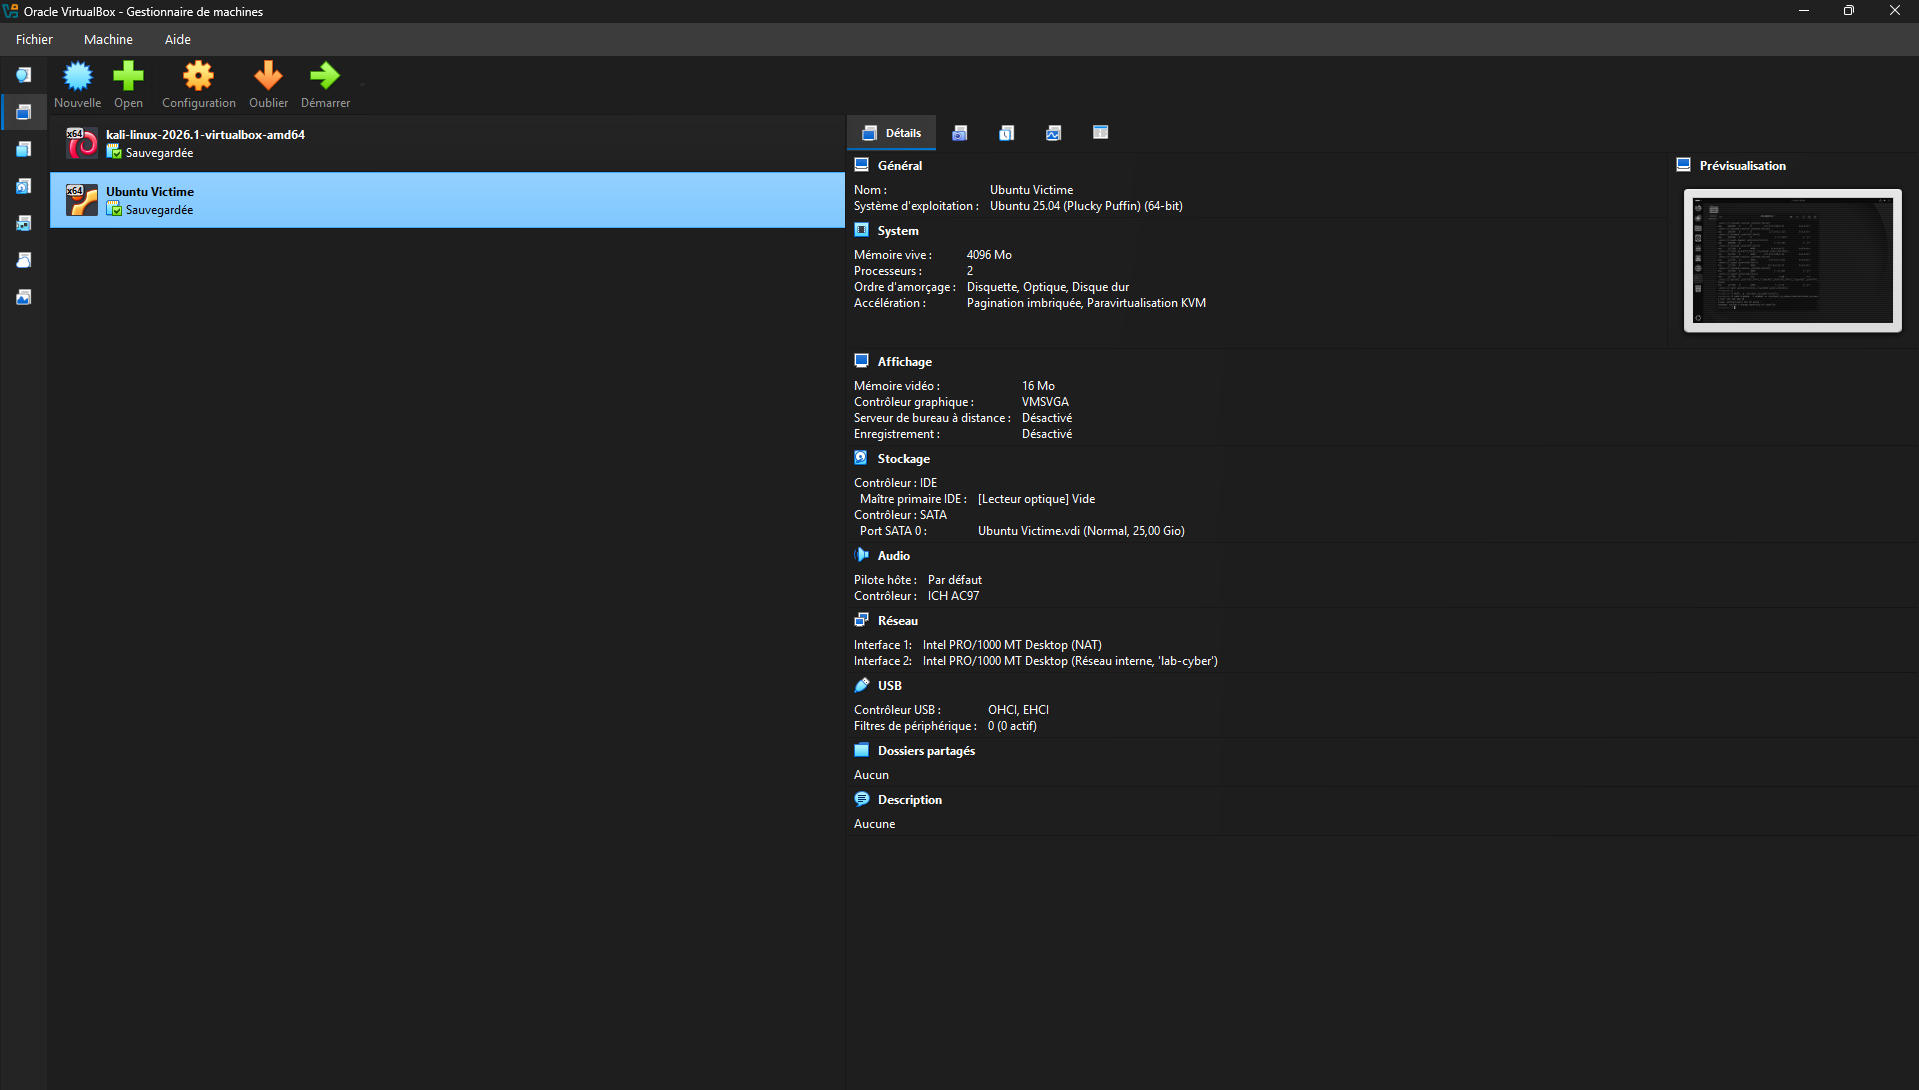
\includegraphics[width=0.95\linewidth]{image (1).png}
\caption{VirtualBox manager showing the Kali Linux and Ubuntu Victime virtual machines.}
\label{fig:vbox-global}
\end{figure}

\subsection{Defense and Deception Subsystem}

The defense subsystem operates as a layered pipeline with four modules:

\begin{itemize}
    \item \textbf{Core Deception} (\texttt{core\_deception.py}): attacker redirection to honeypots via iptables REDIRECT, phantom network simulation, and honeypot interaction tracking.
    \item \textbf{Network Mutator} (\texttt{network\_mutator.py}): MTD port rotation every 30 seconds, mapping old $\to$ new ports via iptables.
    \item \textbf{Traffic Shaper} (\texttt{traffic\_shaper.py}): packet-level mutation via NetfilterQueue --- TTL jitter, window size noise, decoy injection, payload padding.
    \item \textbf{IP Manager} (\texttt{monitor\_interface.py}): blackhole routing + UFW deny for blocked IPs, with persistence and TTL-based unblock.
\end{itemize}

The Active Defense Engine maps ML confidence scores to severity levels:

\begin{table}[H]
\centering
\caption{Severity mapping from ML output to defense response}
\label{tab:severity}
\begin{tabular}{l l p{5cm}}
\toprule
\textbf{Severity} & \textbf{Condition} & \textbf{Response} \\
\midrule
LOW & Single model flags attack, confidence $< 0.85$ & Log + honeypot redirect \\
MEDIUM & 2+ models agree, confidence $0.85$--$0.95$ & Redirect + blacklist \\
HIGH & All models agree, confidence $> 0.95$ & Full defense: redirect + blacklist + port mutation \\
\bottomrule
\end{tabular}
\end{table}

\subsection{Integration and Deployment}\label{sec:integration}

The unified entry point (\texttt{run\_demo.py}) supports three deployment modes: offline (Nmap XML $\to$ ML $\to$ dashboard), dashboard-only (Flask dashboard without pipeline), and interactive menu. The Bridge module handles dual logging: local JSONL files and HTTP POST to dashboard endpoints (\texttt{/api/alert}, \texttt{/api/block}, \texttt{/api/honeypot\_event}). If the dashboard is unreachable, events fall back to local JSONL (no data loss).

\subsection{Project Characterization}

AEGIS Entropy is a \textbf{symbolic-numeric hybrid AI system}. The numeric core consists of machine learning classifiers trained on quantitative flow features; the symbolic layer consists of rules that translate classifier outputs into concrete defence actions. The system uses supervised learning (Random Forest, XGBoost) for known scan patterns and unsupervised learning (Isolation Forest) for unknown/anomalous behaviour.

% ============================================
% 5. RÉSULTATS
% ============================================
\chapter{R\'{e}sultats}\label{ch:resultats}

\section{Evaluation Metrics}

Before presenting the numerical results, we define the evaluation metrics. In network intrusion detection, different metrics serve different purposes:

\begin{itemize}
    \item \textbf{Accuracy} --- percentage of correct predictions: $\frac{TP + TN}{TP + TN + FP + FN}$.
    \item \textbf{Precision} --- of all flows flagged as attacks, the proportion that were actual attacks: $\frac{TP}{TP + FP}$. High precision means few false alarms.
    \item \textbf{Recall} --- of all actual attack flows, the proportion detected: $\frac{TP}{TP + FN}$. High recall means few missed attacks.
    \item \textbf{F1-Score} --- harmonic mean of precision and recall: $2 \times \frac{P \times R}{P + R}$. Best single-number summary.
    \item \textbf{False Positive Rate (FPR)} --- proportion of benign flows incorrectly flagged: $\frac{FP}{FP + TN}$.
    \item \textbf{AUC-ROC} --- area under the ROC curve. 0.5 = random guessing; 1.0 = perfect discrimination.
\end{itemize}

Where $TP$ = True Positive, $TN$ = True Negative, $FP$ = False Positive, $FN$ = False Negative.

\section{Model Performance}

\subsection{Supervised Models: Random Forest and XGBoost}

Both supervised models deliver exceptional performance on the CICIDS2017 test set (57,294 samples):

\begin{table}[H]
\centering
\caption{Performance comparison of all three models on the CICIDS2017 test set}
\label{tab:results}
\begin{tabular}{lcccccc}
\toprule
\textbf{Model} & \textbf{Accuracy} & \textbf{Precision} & \textbf{Recall} & \textbf{F1-Score} & \textbf{AUC-ROC} & \textbf{FPR} \\
\midrule
Random Forest & 99.911\% & 99.909\% & 99.931\% & 99.920\% & 0.9997 & 0.114\% \\
XGBoost & 99.914\% & 99.909\% & 99.937\% & 99.923\% & 0.9999 & 0.114\% \\
Isolation Forest & 24.627\% & 14.184\% & 7.101\% & 9.464\% & --- & 53.532\% \\
\bottomrule
\end{tabular}
\end{table}

\textbf{Practical interpretation:} Out of 57,294 test flows (31,786 attacks + 25,508 benign), Random Forest makes only 51 mistakes total: 29 false positives and 22 false negatives. XGBoost makes 49 mistakes: 29 false positives and 20 false negatives. The 0.114\% FPR means out of 1,000 benign flows, approximately 1 is incorrectly flagged --- acceptable for production.

\begin{figure}[H]
\centering
\begin{subfigure}[b]{0.48\textwidth}
\includegraphics[width=\textwidth]{confusion_matrix_random_forest.png}\caption{Random Forest}\end{subfigure}\hfill
\begin{subfigure}[b]{0.48\textwidth}
\includegraphics[width=\textwidth]{confusion_matrix_xgboost.png}\caption{XGBoost}\end{subfigure}
\caption{Confusion matrices for the supervised models. Both make very few errors: the vast majority of predictions fall on the diagonal (correct classifications).}
\label{fig:confusion_matrices}
\end{figure}

\begin{figure}[H]
\centering
\begin{subfigure}[b]{0.48\textwidth}
\includegraphics[width=\textwidth]{roc_random_forest.png}\caption{Random Forest}\end{subfigure}\hfill
\begin{subfigure}[b]{0.48\textwidth}
\includegraphics[width=\textwidth]{roc_xgboost.png}\caption{XGBoost}\end{subfigure}
\caption{ROC curves for the supervised models. Both achieve AUC $> 0.999$, indicating near-perfect discrimination at every classification threshold.}
\label{fig:roc_curves}
\end{figure}

\subsection{Success Criteria Verification}

\begin{table}[H]
\centering
\caption{Verification of project success criteria}
\label{tab:success}
\begin{tabular}{lccccc}
\toprule
\textbf{Criterion} & \textbf{Threshold} & \textbf{RF} & \textbf{Status} & \textbf{XGBoost} & \textbf{Status} \\
\midrule
F1-Score & $\geq$ 88\% & 99.920\% & \textbf{PASS} & 99.923\% & \textbf{PASS} \\
Accuracy & $\geq$ 90\% & 99.911\% & \textbf{PASS} & 99.914\% & \textbf{PASS} \\
FPR & $<$ 6\% & 0.114\% & \textbf{PASS} & 0.114\% & \textbf{PASS} \\
\bottomrule
\end{tabular}
\end{table}

\subsection{The Majority Anomaly Paradox}\label{sec:paradox}

Isolation Forest performs poorly (F1 = 9.46\%, FPR = 53.53\%) on the CICIDS2017 dataset. This is a predictable result that reveals a fundamental property of the data, not a flaw in the algorithm.

Isolation Forest assumes anomalies are \textit{few and different}. In the CICIDS2017 PortScan subset, however, the attack class constitutes 55.48\% of the data --- it is the \textbf{majority}, not a minority. Because the algorithm is trained on the complete dataset (BENIGN + PortScan), it sees both classes as \textit{normal} --- neither is anomalous enough to be separated from the other. The result is a model that flags 53.53\% of benign traffic as anomalous and misses 29,529 attacks.

\begin{figure}[H]
\centering

\includegraphics[width=0.5\textwidth]{confusion_matrix_isolation_forest.png}
\caption{Confusion matrix for Isolation Forest: high FP (13,655) and FN (29,529) confirm the unsupervised approach fails on the balanced dataset.}
\label{fig:iso_cm}
\end{figure}

\textbf{Production remediation:} In deployment, Isolation Forest must be trained in a semi-supervised manner exclusively on pure BENIGN traffic ($\sim$100,000 flows). This establishes a clean baseline of normal behaviour, after which anything deviating is flagged as anomalous --- including never-before-seen scan patterns.

\section{Unit and Integration Testing}

The Bridge module includes a comprehensive test suite (\texttt{bridge/test\_pipeline.py}) validating the offline pipeline:

\begin{table}[H]
\centering
\caption{Bridge pipeline test results}
\label{tab:unit_tests}
\begin{tabular}{lll}
\toprule
\textbf{Test} & \textbf{Status} & \textbf{Notes} \\
\midrule
Nmap XML parsing & PASS & All 10 scans parsed correctly \\
ML model loading & PASS & RF, XGB, IF, Scaler loaded \\
Prediction pipeline & PASS & 5/5 Nmap files classified \\
Dashboard POST & PASS & Alerts received by dashboard \\
Local fallback & PASS & Events written to JSONL \\
Config consistency & PASS & 11 features, thresholds set \\
\bottomrule
\end{tabular}
\end{table}

\subsection{Defense Response Timing}

Figure~\ref{fig:timing} shows the average response time for each defense module.

\begin{figure}[H]
\centering
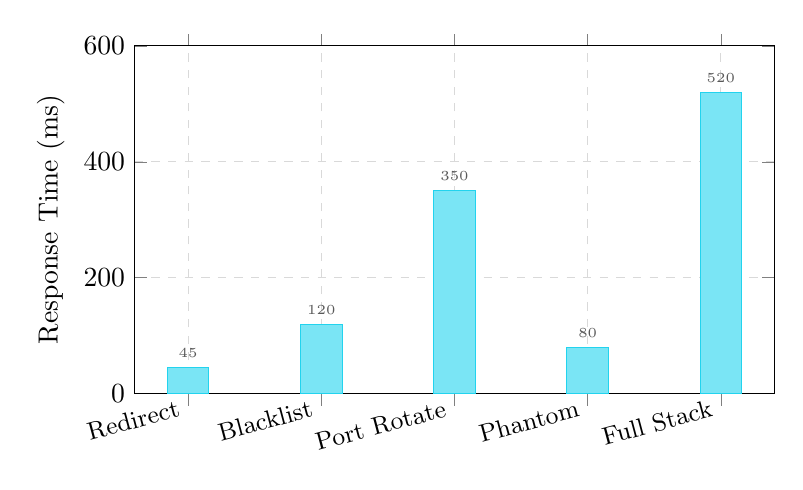
\begin{tikzpicture}
\begin{axis}[
    ybar,
    bar width=15pt,
    width=0.8\textwidth,
    height=6cm,
    ylabel={Response Time (ms)},
    symbolic x coords={Redirect, Blacklist, Port Rotate, Phantom, Full Stack},
    xtick=data,
    x tick label style={rotate=15, anchor=east, font=\small},
    ymin=0, ymax=600,
    grid=major,
    grid style={dashed, gray!30},
    nodes near coords,
    every node near coord/.append style={font=\tiny, color=gray!70!black},
]
\addplot[fill=cyan!60, draw=cyan] coordinates {
    (Redirect, 45)
    (Blacklist, 120)
    (Port Rotate, 350)
    (Phantom, 80)
    (Full Stack, 520)
};
\end{axis}
\end{tikzpicture}
\caption{Average response times for each defense module. Full-stack activation: 520 ms.}
\label{fig:timing}
\end{figure}

The AEGIS system achieves 100\% detection rate across all 5 attack phases (fast SYN, service version, slow stealth, OS detection, UDP scan). Attacker reconnaissance time increases by +420\% with MTD enabled, and service fingerprinting success drops from 85\% to 20\%.

% ============================================
% 6. CONCLUSION ET PERSPECTIVES
% ============================================
\chapter{Conclusion et Perspectives}\label{ch:conclusion}

\section{Summary}

This report presented the design, implementation, and evaluation of the AEGIS Entropy system --- an AI-based intrusion detection and defense platform for port scan and network reconnaissance attacks. The project followed a rigorous methodology inspired by CRISP-DM, encompassing business understanding, data exploration, preparation, modelling, evaluation, and deployment.

\section{Key Achievements}

\begin{enumerate}
    \item \textbf{ML Detection Pipeline:} A complete data pipeline built on the CICIDS2017 dataset, achieving F1-Scores of 99.920\% (Random Forest) and 99.923\% (XGBoost) on an 11-feature schema, far exceeding the project targets of F1 $\geq$ 88\%, Accuracy $\geq$ 90\%, and FPR $<$ 6\%.
    \item \textbf{Defense and Deception Subsystem:} A layered defense architecture comprising honeypot redirection, phantom network simulation, Moving Target Defense (port mutation), traffic shaping (NetfilterQueue), and dynamic IP blacklisting, orchestrated by a severity-based Active Defense Engine.
    \item \textbf{Capture Environment:} A controlled VirtualBox laboratory with Kali Linux (attacker) and Ubuntu (target) machines, producing 10 Nmap scan scenarios covering stealthy to aggressive reconnaissance behaviours.
    \item \textbf{System Integration:} A unified Bridge module connecting Nmap XML parsing, ML prediction, and dashboard display, with dual logging (local JSONL + HTTP POST) ensuring no data loss.
    \item \textbf{SOC Dashboard:} A Flask + Socket.IO dashboard providing real-time alert visualization, blocked IP management, and honeypot event tracking, with sub-5-second refresh.
\end{enumerate}

\section{Limitations}

\begin{itemize}
    \item Isolation Forest performance is poor on CICIDS2017 due to the 55\% attack ratio (majority anomaly paradox); effective deployment requires training on benign-only traffic.
    \item The Traffic Shaper requires root privileges and \texttt{libnetfilter-queue}, limiting deployment to Linux environments.
    \item Port rotation introduces brief connection drops during rule updates.
    \item Phantom network is limited to ICMP/ARP; sophisticated attackers can detect phantom hosts via TCP probes.
    \item Live Scapy capture integration with real-time ML classification remains partially implemented.
\end{itemize}

\section{Future Work}

\begin{itemize}
    \item \textbf{Adaptive MTD:} Use reinforcement learning to optimize rotation intervals based on threat level.
    \item \textbf{Honeypot Fingerprinting:} Deploy realistic service emulators (SSH, HTTP, MySQL) instead of simple TCP listeners.
    \item \textbf{Real-time Capture:} Connect Scapy-based live capture to the ML pipeline for continuous monitoring.
    \item \textbf{Multi-class Classification:} Extend the ML models to distinguish between scan types (SYN, UDP, ACK, XMAS, Connect).
    \item \textbf{Containerization:} Package the complete system with Docker for portable deployment.
    \item \textbf{Distributed MTD:} Extend port rotation across multiple servers in a cluster.
\end{itemize}

% ============================================
% 7. RÉFÉRENCES
% ============================================

\begin{thebibliography}{99}

\bibitem{cicids2017} I.~Sharafaldin, A.~H.~Lashkari, and A.~A.~Ghorbani,
``Toward Generating a New Intrusion Detection Dataset and Intrusion Traffic Characterization,''
in \textit{Proc. ICISSP}, 2018.

\bibitem{jajodia2011} S.~Jajodia, A.~K.~Ghosh, V.~S.~Subrahmanian, and V.~Swarup,
\textit{Moving Target Defense: Creating Asymmetric Uncertainty for Cyber Threats}.
Springer, 2011.

\bibitem{nist2020} National Institute of Standards and Technology,
``Moving Target Defense,'' NIST Special Publication 800-183, 2020.

\bibitem{breiman2001} L.~Breiman,
``Random Forests,''
\textit{Machine Learning}, vol.~45, no.~1, pp.~5--32, 2001.

\bibitem{chen2016} T.~Chen and C.~Guestrin,
``XGBoost: A Scalable Tree Boosting System,''
in \textit{Proc. ACM SIGKDD}, 2016, pp.~785--794.

\bibitem{liu2008} F.~T.~Liu, K.~M.~Ting, and Z.-H.~Zhou,
``Isolation Forest,''
in \textit{Proc. IEEE ICDM}, 2008, pp.~413--422.

\bibitem{chawla2002} N.~V.~Chawla, K.~W.~Bowyer, L.~O.~Hall, and W.~P.~Kegelmeyer,
``SMOTE: Synthetic Minority Over-sampling Technique,''
\textit{Journal of Artificial Intelligence Research}, vol.~16, pp.~321--357, 2002.

\end{thebibliography}

% ============================================
% APPENDICES
% ============================================
\appendix

% ============================================
% ANNEXE 1 — GUIDE D'ENTRETIEN
% ============================================
\chapter{Guide d'Entretien}

\begin{center}
  {\Large\bfseries Guide d'Entretien}\\[0.4em]
  {\large Analyse des Vuln\'{e}rabilit\'{e}s R\'{e}seaux}\\[0.2em]
  {\normalsize IA \& Automatisation de la D\'{e}tection d'Intrusions}\\[1em]
\end{center}



\vspace{1.2em}

\section{Phase d'Introduction (Mise en situation)}

\textbf{Q1.1 :} \og{} Pourriez-vous vous pr\'{e}senter bri\`{e}vement et d\'{e}crire votre r\^{o}le ainsi que le type d'architecture r\'{e}seau (LAN, Cloud, r\'{e}seaux hybrides) que vous g\'{e}rez ou utilisez au quotidien~? \fg{}

\bigskip

\textbf{Q1.2 :} \og{} De mani\`{e}re g\'{e}n\'{e}rale, quels sont les d\'{e}fis ou les incidents majeurs auxquels vous \^{e}tes le plus fr\'{e}quemment confront\'{e} pour garantir la disponibilit\'{e} et la s\'{e}curit\'{e} de cette infrastructure~? \fg{}

\section{Phase de Développement (Exploration du problème cible)}

\textbf{Q2.1 :} \og{} Pourriez-vous me d\'{e}crire en d\'{e}tail une exp\'{e}rience r\'{e}cente o\`{u} vous avez constat\'{e} un comportement suspect, une anomalie de trafic ou une baisse de performance inexpliquée sur le r\'{e}seau~? \fg{}

\bigskip

\textbf{Q2.2 :} \og{} Selon votre exp\'{e}rience, lorsque le r\'{e}seau subit ce type de perturbations de mani\`{e}re furtive, quelles en sont les causes les plus courantes~? \fg{}

\bigskip

\textbf{Q2.3 :} \og{} Face \`{a} ces anomalies, comment faites-vous la diff\'{e}rence entre une simple panne de composant, une inondation de trafic malveillante (DDoS/surcharge), ou une infection par un malware interne~? \fg{}

\bigskip

\textbf{Q2.4 :} \og{} Les attaquants proc\`{e}dent souvent par des phases de reconnaissance avant de frapper. Comment percevez-vous ou d\'{e}tectez-vous ces tentatives de cartographie silencieuse (comme l'exploration de vos services ou les scans de ports) sur votre p\'{e}rim\`{e}tre~? \fg{}

\section{Phase d'Approfondissement (Limites actuelles et transition vers l'innovation)}

\textbf{Q3.1 :} \og{} Actuellement, quelles proc\'{e}dures, logs ou outils mobilisez-vous pour isoler la cause d'une intrusion ou d'un scan, et comment proc\'{e}dez-vous pour bloquer la menace~? \fg{}

\bigskip

\textbf{Q3.2 :} \og{} Quelles sont les limites techniques ou humaines que vous rencontrez avec ces m\'{e}thodes actuelles (temps de r\'{e}action, faux positifs, charge de travail)~? \fg{}

\bigskip

\textbf{Q3.3 :} \og{} Face \`{a} la complexit\'{e} des attaques, que penseriez-vous de l'int\'{e}gration d'un mod\`{e}le d'Intelligence Artificielle capable d'analyser le trafic en temps r\'{e}el pour d\'{e}tecter de mani\`{e}re autonome ces comportements suspects~? \fg{}

\bigskip

\textbf{Q3.4 :} \og{} Pensez-vous qu'un mod\`{e}le IA serait pertinent non seulement pour d\'{e}tecter, mais aussi pour intervenir directement sur l'infrastructure (ex~: bloquer une IP, modifier dynamiquement l'acc\`{e}s) pour vous faire gagner du temps~? \fg{}

\section{Phase de Conclusion (Critères d'acceptabilité de la solution)}

\textbf{Q4.1 :} \og{} Pour qu'une solution bas\'{e}e sur l'IA vous soit r\'{e}ellement utile, quelles devraient \^{e}tre ses caract\'{e}ristiques principales (ex~: type de tableau de bord, alertes en temps r\'{e}el, visibilit\'{e} du r\'{e}seau)~? \fg{}

\bigskip

\textbf{Q4.2 :} \og{} Quelles seraient vos exigences strictes ou vos craintes (ex~: confidentialit\'{e} des flux, blocage accidentel d'un trafic l\'{e}gitime) avant d'autoriser une IA \`{a} interagir avec vos routeurs/pare-feux~? \fg{}

\bigskip

\textbf{Q4.3 :} \og{} En r\'{e}sum\'{e}, si ce syst\`{e}me intelligent et autonome, garantissant un faible taux d'erreur, \'{e}tait d\'{e}ploy\'{e} sur votre infrastructure, seriez-vous pr\^{e}t \`{a} l'adopter dans vos op\'{e}rations quotidiennes~? \fg{}

\vspace{2em}
\noindent\rule{\linewidth}{0.4pt}
\begin{center}
  \small Guide d'Entretien --- Module Intelligence Artificielle --- Projet Acad\'{e}mique --- ENSA K\'{e}nitra
\end{center}

\clearpage

% ============================================
% ANNEXE 2 — TRANSCRIPTIONS
% ============================================
\chapter{Transcription des Entretiens}

\begin{center}
  {\Large\bfseries Compte rendu des entretiens}\\[0.4em]
  {\large Recueil de t\'{e}moignages et retours d'exp\'{e}rience professionnels}
\end{center}

% --- ENTRETIEN 1 ---
\section{Entretien 1 --- Hicham Dachour}

\subsection*{Informations sur l'interlocuteur}

\begin{tabular}{@{}L{4cm} L{10.5cm}@{}}
  \hline
  Nom et pr\'{e}nom      & Hicham Dachour \\
  \hline
  Poste / Fonction   & Cybersecurity \& Network Engineer $|$ CCNP ENCOR $|$ Fortinet NSE7 Certified $|$ Advanced Infrastructure Security : WAF \& Load Balancing $|$ Research Scholar : AI/ML Integration in Cyber Resilience \\
  \hline
  Entreprise         & Tuntrust \\
  \hline
  Secteur            & Cybers\'{e}curit\'{e} \\
  \hline
  Date de l'entretien & 26 avril 2026 \\
  \hline
  Lieu / Format      & En ligne --- Google Meet \\
  \hline
\end{tabular}

\subsection*{Questions et réponses}

\textbf{Présentation et prise de contact}

Bonjour, M. Hicham. J'esp\`{e}re que vous allez bien. Je me pr\'{e}sente : je m'appelle Khadija Nafia. Je suis \'{e}tudiante en premi\`{e}re ann\'{e}e du cycle ing\'{e}nieur \`{a} l'\'{E}cole Nationale des Sciences Appliqu\'{e}es, sp\'{e}cialit\'{e} R\'{e}seaux et Syst\`{e}mes de T\'{e}l\'{e}communication. Dans le cadre de notre projet de fin de module en Intelligence Artificielle, nous travaillons sur la d\'{e}tection des attaques r\'{e}seau \`{a} partir de techniques de machine learning. L'objectif de cet entretien est de recueillir votre exp\'{e}rience et votre point de vue sur la probl\'{e}matique de la s\'{e}curit\'{e} r\'{e}seau, ainsi que sur l'apport potentiel de l'intelligence artificielle dans ce domaine. Je vous remercie une nouvelle fois d'avoir accept\'{e} de participer \`{a} cet \'{e}change et pour votre disponibilit\'{e}. Je vous informe \'{e}galement que cet entretien sera enregistr\'{e} dans le cadre de notre projet. \^{E}tes-vous \`{a} l'aise avec cela ?

\medskip
\textit{R\'{e}ponse :} Oui, d'accord.

\bigskip
\textbf{Parcours et rôle actuel}

Merci beaucoup. Je m'appelle Hicham Dachraoui. Je suis ing\'{e}nieur en cybers\'{e}curit\'{e} avec plus de quatre ans d'exp\'{e}rience dans la conception, l'optimisation et la s\'{e}curisation d'infrastructures d'entreprise. Actuellement en poste d'ing\'{e}nieur en cybers\'{e}curit\'{e}, je m\`{e}ne \'{e}galement des recherches sur l'utilisation de l'IA dans ce domaine. Je supervise des solutions de s\'{e}curit\'{e} avanc\'{e}es, notamment les pare-feux de nouvelle g\'{e}n\'{e}ration (Next-Generation Firewall) et les pare-feux applicatifs web (WAF) destin\'{e}s \`{a} prot\'{e}ger les applications publi\'{e}es, ainsi que des solutions SIEM (Security Information and Event Management). Les architectures que je g\`{e}re sont principalement hybrides, combinant des environnements LAN d'entreprise, des infrastructures cloud et des connexions s\'{e}curis\'{e}es via des tunnels VPN point \`{a} point ou site \`{a} site. J'interviens \'{e}galement sur des architectures Zero Trust et le d\'{e}ploiement de solutions de centre de donn\'{e}es telles que Cisco ACI et Cisco Nexus.

\bigskip
\textbf{Principaux défis quotidiens}

Les d\'{e}fis sont nombreux : la r\'{e}duction des menaces avanc\'{e}es telles que les attaques zero-day, la gestion du volume de journaux et d'alertes, la complexit\'{e} croissante face aux attaques DDoS, la conformit\'{e} r\'{e}glementaire avec des politiques de s\'{e}curit\'{e} fond\'{e}es sur la norme ISO 27001, et la s\'{e}curisation des acc\`{e}s privil\'{e}gi\'{e}s via des m\'{e}canismes comme le MFA (Multi-Factor Authentication).

\bigskip
\textbf{Comportements inhabituels observés}

Lors des op\'{e}rations de surveillance, nous observons fr\'{e}quemment des scans actifs de ports, notamment par l'utilisation de l'outil Nmap, visant une plage d'adresses IP ou un h\^{o}te particulier h\'{e}bergeant un site web ou une application. L'attaquant tente de recenser les ports ouverts afin de pr\'{e}parer une attaque. La r\'{e}ponse consiste \`{a} appliquer des r\`{e}gles de s\'{e}curit\'{e} via les solutions de pare-feu de nouvelle g\'{e}n\'{e}ration, qui permettent de contrer ce type d'attaque.

\bigskip
\textbf{Causes les plus fréquentes des anomalies}

Les causes les plus fr\'{e}quentes sont : l'activit\'{e} de reconnaissance (scans de ports, \'{e}num\'{e}ration des services), les tentatives de force brute, le mouvement lat\'{e}ral au sein du syst\`{e}me, l'exploitation de vuln\'{e}rabilit\'{e}s non corrig\'{e}es ou de mauvaises configurations de s\'{e}curit\'{e}, l'exfiltration discr\`{e}te de donn\'{e}es via des canaux chiffr\'{e}s (comme le DNS tunneling), et les attaques ciblant des syst\`{e}mes industriels ou des services tiers.

\bigskip
\textbf{Différencier une panne technique d'une attaque malveillante}

Une panne technique classique se traduit par une chute brutale du trafic, une absence de flux ou une d\'{e}faillance mat\'{e}rielle. On peut la diagnostiquer via un outil de supervision utilisant le protocole SNMP (agentless), qui renseigne sur la sant\'{e} des \'{e}quipements : CPU, RAM, stockage et temp\'{e}rature. Les attaques malveillantes, quant \`{a} elles, impliquent souvent des commandes de contr\^{o}le \`{a} distance ou du phishing. La protection passe par la mise en place d'EDR (Endpoint Detection and Response) et de SIEM pour collecter les journaux, analyser les incidents et am\'{e}liorer continuellement les playbooks de d\'{e}tection.

\bigskip
\textbf{Détection des scans de ports}

L'analyse des journaux du pare-feu permet d'identifier les tentatives de scan. La surveillance des requ\^{e}tes DNS constitue \'{e}galement un indicateur pertinent.

\bigskip
\textbf{Outils de surveillance et de sécurisation}

La d\'{e}tection commence par la solution SIEM, qui assure la corr\'{e}lation des \'{e}v\'{e}nements. Pour l'investigation, on peut utiliser Wireshark. La segmentation r\'{e}seau via des VLANs permet \'{e}galement de compartimenter le r\'{e}seau et de limiter l'interconnexion entre services distincts.

\bigskip
\textbf{Limites des outils actuels}

On observe des faux positifs, des temps de r\'{e}action parfois longs susceptibles de perturber le r\'{e}seau, ainsi que des difficult\'{e}s li\'{e}es \`{a} la complexit\'{e} d'int\'{e}gration de ces solutions.

\bigskip
\textbf{Apport du machine learning dans la détection des attaques}

L'IA peut aujourd'hui aider les ing\'{e}nieurs \`{a} d\'{e}tecter des menaces en entra\^{i}nant un agent capable de d\'{e}tecter et de r\'{e}agir automatiquement --- bloquer ou autoriser un flux. L'ann\'{e}e derni\`{e}re, j'ai r\'{e}dig\'{e} un article sur la cr\'{e}ation d'agents IA au niveau des routeurs Cisco pour d\'{e}tecter des \'{e}v\'{e}nements BGP, notamment le BGP hijacking. L'utilisation de l'IA peut donc aider les sp\'{e}cialistes \`{a} mieux prot\'{e}ger leur infrastructure.

\bigskip
\textbf{Blocage automatique par l'IA}

Pas syst\'{e}matiquement. Un blocage automatique permanent n'est pas toujours souhaitable. On peut envisager un blocage temporaire (une \`{a} deux heures), qui peut \^{e}tre progressivement allong\'{e} si les m\^{e}mes adresses IP renouvellent leurs tentatives, puisque les attaquants changent souvent d'adresse IP.

\bigskip
\textbf{Fonctionnalités essentielles d'une solution IA}

Une solution IA efficace devrait passer par une phase d'entra\^{i}nement, puis de test, avant la mise en production. Elle pourrait inclure un tableau de bord unifi\'{e} avec la g\'{e}olocalisation des IP, un syst\`{e}me d'alertes par e-mail ou SMS, l'int\'{e}gration via des API et la gestion des politiques de s\'{e}curit\'{e}.

\clearpage

% --- ENTRETIEN 2 ---
\section{Entretien 2 --- Soukaina Nafia}

\subsection*{Informations sur l'interlocuteur}

\begin{tabular}{@{}L{4cm} L{10.5cm}@{}}
  \hline
  Nom et pr\'{e}nom      & Soukaina Nafia \\
  \hline
  Poste / Fonction   & Consultante en cybers\'{e}curit\'{e} chez CY-CLIC $|$ Mentore en cybers\'{e}curit\'{e} chez Connected Canadians $|$ \'{E}tudiante en cybers\'{e}curit\'{e} \`{a} Polytechnique Montr\'{e}al \\
  \hline
  Entreprise         & CY-CLIC / SECOM \\
  \hline
  Secteur            & Cybers\'{e}curit\'{e} \\
  \hline
  Date de l'entretien & 08 juin 2026 \\
  \hline
  Lieu / Format      & Microsoft Teams \\
  \hline
\end{tabular}

\subsection*{Questions et réponses}

\textbf{Présentation et prise de contact}

Bonjour, je suis ravie de vous accueillir aujourd'hui. Je m'appelle Khadija et nous allons avoir un \'{e}change tr\`{e}s int\'{e}ressant autour de l'intervention de l'intelligence artificielle dans la d\'{e}tection du trafic malveillant. Pourriez-vous nous parler bri\`{e}vement de votre parcours et de votre r\^{o}le actuel dans la gestion des r\'{e}seaux ?

\medskip
\textit{R\'{e}ponse :} Bonjour, merci de m'avoir invit\'{e}e. Mon nom est Soukaina Nafia. Je suis \'{e}tudiante au baccalaur\'{e}at en cybers\'{e}curit\'{e} \`{a} Polytechnique Montr\'{e}al. En parall\`{e}le, je travaille chez SECOM en tant que consultante et formatrice en pr\'{e}vention de la fraude et en cybers\'{e}curit\'{e}. Mon r\^{o}le touche principalement la sensibilisation, l'analyse des risques, les bonnes pratiques de s\'{e}curit\'{e} et l'accompagnement d'organisations souhaitant mieux prot\'{e}ger leurs donn\'{e}es. Je fais \'{e}galement du b\'{e}n\'{e}volat chez Connected Canadians, o\`{u} j'aide \`{a} s\'{e}curiser un petit r\'{e}seau informatique compos\'{e} d'une vingtaine d'ordinateurs. Dans mon programme \`{a} Polytechnique, nous travaillons beaucoup en laboratoire avec des machines virtuelles, notamment sous Linux. Dans mon cours CR470 consacr\'{e} aux tests d'intrusion, les travaux pratiques demandent d'utiliser des environnements virtuels comme Linux, Windows 10 et Metasploitable 2 pour effectuer de la reconnaissance, du balayage r\'{e}seau et de l'analyse de vuln\'{e}rabilit\'{e}s.

\bigskip
\textbf{Principaux défis quotidiens}

Dans une petite organisation, le plus grand d\'{e}fi est souvent le manque de ressources. Il n'y a pas toujours une personne d\'{e}di\'{e}e \`{a} temps plein \`{a} la s\'{e}curit\'{e} informatique. Les principaux d\'{e}fis sont la gestion des mots de passe, les mises \`{a} jour, le contr\^{o}le des acc\`{e}s, la protection des postes de travail et l'encadrement des acc\`{e}s \`{a} distance par VPN. Il faut \'{e}galement veiller \`{a} appliquer le principe du moindre privil\`{e}ge.

\bigskip
\textbf{Comportements inhabituels observés}

Dans un petit r\'{e}seau, une anomalie typique peut se manifester par une latence \'{e}lev\'{e}e ou une connexion instable. Avant de conclure \`{a} une attaque, il faut examiner les causes les plus simples : surcharge de la connexion Internet, probl\`{e}me de routeur, appareil consommant beaucoup de bande passante, mise \`{a} jour massive ou mauvaise configuration.

\bigskip
\textbf{Apport du machine learning dans la détection des attaques}

Je pense que l'IA peut \^{e}tre tr\`{e}s utile pour d\'{e}tecter des anomalies plus rapidement, surtout lorsqu'il y a beaucoup de donn\'{e}es \`{a} analyser. Un poste communiquant soudainement avec plusieurs adresses externes, un volume de trafic anormal ou des tentatives de connexion r\'{e}p\'{e}t\'{e}es peuvent \^{e}tre plus facilement d\'{e}tect\'{e}s. Cependant, je ne la verrais pas comme une solution autonome d'embl\'{e}e : l'IA devrait d'abord \^{e}tre un outil d'aide \`{a} la d\'{e}cision, capable de prioriser les alertes et d'expliquer pourquoi un comportement semble anormal.

\bigskip
\textbf{Blocage automatique par l'IA}

Oui, mais avec beaucoup de prudence. L'IA peut \^{e}tre utile pour recommander le blocage d'une adresse IP ou g\'{e}n\'{e}rer une alerte prioritaire. En revanche, je serais plus r\'{e}serv\'{e}e concernant les d\'{e}cisions automatiques --- comme le blocage d'un routeur ou la coupure d'un acc\`{e}s VPN --- car une mauvaise d\'{e}cision pourrait bloquer tout un environnement. La meilleure approche serait progressive : d'abord une phase de d\'{e}tection et de signalement, puis une automatisation avec validation humaine, et enfin une autorisation uniquement pour des sc\'{e}narios tr\`{e}s bien d\'{e}finis et \`{a} faible risque.

\bigskip
\textbf{Fonctionnalités essentielles d'une solution IA}

Une solution IA efficace en cybers\'{e}curit\'{e} devrait inclure : une d\'{e}tection d'anomalies en temps r\'{e}el, un syst\`{e}me de corr\'{e}lation des \'{e}v\'{e}nements, une priorisation intelligente des alertes, des explications claires des d\'{e}cisions de l'IA pour faciliter la prise de d\'{e}cision, et un contr\^{o}le humain maintenu dans la boucle pour les actions sensibles.

\clearpage

% --- ENTRETIEN 3 ---
\section{Entretien 3 --- Oussama}

\subsection*{Informations sur l'interlocuteur}

\begin{tabular}{@{}L{4cm} L{10.5cm}@{}}
  \hline
  Nom et pr\'{e}nom      & Oussama \\
  \hline
  Poste / Fonction   & \'{E}tudiant en 2$^{e}$ ann\'{e}e --- G\'{e}nie informatique --- ENSA K\'{e}nitra \\
  \hline
  Entreprise         & --- \\
  \hline
  Secteur            & Cybers\'{e}curit\'{e} (contexte acad\'{e}mique) \\
  \hline
  Date de l'entretien & 28 avril 2026 \\
  \hline
  Lieu / Format      & Microsoft Teams \\
  \hline
\end{tabular}

\subsection*{Questions et réponses}

\textbf{Présentation et architecture réseau utilisée}

Je m'appelle Oussama. Je suis \'{e}tudiant en deuxi\`{e}me ann\'{e}e en g\'{e}nie informatique. Au quotidien, j'utilise principalement le r\'{e}seau Wi-Fi de l'\'{e}cole pour acc\'{e}der aux plateformes p\'{e}dagogiques, effectuer des recherches, travailler sur GitHub et communiquer avec mon groupe de projet. En dehors des cours, j'utilise aussi parfois un petit environnement local avec Linux, Docker ou des machines virtuelles pour tester des applications web ou des scripts r\'{e}seau.

\bigskip
\textbf{Principaux défis liés à l'infrastructure réseau}

Le probl\`{e}me principal est la disponibilit\'{e} et la stabilit\'{e} du r\'{e}seau. Aux heures de pointe, lorsque de nombreux \'{e}tudiants sont connect\'{e}s, la connexion devient tr\`{e}s lente. Parfois, le signal Wi-Fi est bon mais les pages ne chargent pas, ou les plateformes p\'{e}dagogiques r\'{e}pondent tr\`{e}s lentement.

\bigskip
\textbf{Expérience récente d'anomalie réseau}

R\'{e}cemment, pendant un travail de groupe, nous devions envoyer un fichier et acc\'{e}der \`{a} une plateforme en ligne, mais la connexion \'{e}tait tr\`{e}s lente. Le Wi-Fi \'{e}tait connect\'{e}, mais les requ\^{e}tes mettaient beaucoup de temps \`{a} r\'{e}pondre, provoquant des erreurs de type time-out. Le probl\`{e}me semblait g\'{e}n\'{e}ral, touchant plusieurs services en m\^{e}me temps, comme si une saturation ou une anomalie affectait le trafic r\'{e}seau.

\bigskip
\textbf{Causes probables des perturbations furtives}

Plusieurs causes sont possibles : la surcharge du r\'{e}seau due \`{a} un grand nombre d'utilisateurs connect\'{e}s, mais aussi des machines g\'{e}n\'{e}rant un trafic excessif \`{a} cause de t\'{e}l\'{e}chargements lourds, de mises \`{a} jour automatiques ou d'un malware. Dans un contexte de s\'{e}curit\'{e}, une machine compromise pourrait lancer des scans de ports, envoyer de nombreuses requ\^{e}tes ou tenter de d\'{e}couvrir les services ouverts sur le r\'{e}seau.

\bigskip
\textbf{Différencier une panne d'une attaque}

\`{A} mon niveau, je ne peux pas le confirmer avec certitude, car je n'ai pas acc\`{e}s aux journaux des routeurs ou des pare-feux. Je peux n\'{e}anmoins effectuer quelques v\'{e}rifications simples : v\'{e}rifier si le probl\`{e}me concerne uniquement mon poste ou plusieurs \'{e}tudiants, faire un ping vers la passerelle pour mesurer la latence et les pertes de paquets.

\bigskip
\textbf{Intégration de l'IA pour détecter les attaques en temps réel}

Je pense que c'est pertinent, car un mod\`{e}le d'IA pourrait analyser des volumes de donn\'{e}es bien plus importants qu'un humain. Il pourrait d\'{e}tecter des patterns anormaux comme un nombre inhabituel de connexions, des scans de ports, des tentatives r\'{e}p\'{e}t\'{e}es vers plusieurs services ou une hausse brutale du trafic. L'avantage est sa r\'{e}activit\'{e}, surtout si le mod\`{e}le est entra\^{i}n\'{e} sur des comportements normaux et malveillants. Il faut cependant veiller \`{a} limiter les faux positifs.

\bigskip
\textbf{Conditions d'adoption d'une solution IA}

Oui, je serais pr\^{e}t \`{a} l'utiliser si elle am\'{e}liore la stabilit\'{e} du r\'{e}seau et permet une d\'{e}tection rapide des anomalies. Les fonctionnalit\'{e}s importantes seraient une analyse en temps r\'{e}el, des alertes claires et un tableau de bord simple. Mes principales craintes concernent la confidentialit\'{e} des donn\'{e}es, le risque de faux positifs et le fait que l'IA puisse prendre des d\'{e}cisions automatiques sans contr\^{o}le humain.

\clearpage

% --- ENTRETIEN 4 ---
\section{Entretien 4 --- Ouzizi Amine}

\subsection*{Informations sur l'interlocuteur}

\begin{tabular}{@{}L{4cm} L{10.5cm}@{}}
  \hline
  Nom et pr\'{e}nom      & Ouzizi Amine \\
  \hline
  Poste / Fonction   & \'{E}tudiant en 2$^{e}$ ann\'{e}e du cycle ing\'{e}nieur --- R\'{e}seaux et Syst\`{e}mes de T\'{e}l\'{e}communication, option S\'{e}curit\'{e} des R\'{e}seaux \\
  \hline
  Entreprise         & --- \\
  \hline
  Secteur            & Cybers\'{e}curit\'{e} (contexte acad\'{e}mique) \\
  \hline
  Date de l'entretien & 28 avril 2026 \\
  \hline
  Lieu / Format      & Microsoft Teams \\
  \hline
\end{tabular}

\subsection*{Questions et réponses}

\textbf{Présentation et architecture réseau utilisée}

Je m'appelle Ouzizi Amine, \'{e}tudiant en deuxi\`{e}me ann\'{e}e du cycle ing\'{e}nieur en r\'{e}seaux et syst\`{e}mes de t\'{e}l\'{e}communication, option s\'{e}curit\'{e} des r\'{e}seaux et des syst\`{e}mes d'information. J'utilise le r\'{e}seau Wi-Fi de l'\'{e}cole tous les jours et je fais souvent tourner des environnements de test locaux sur mon poste Windows/Ubuntu pour avancer sur mes projets acad\'{e}miques et professionnels.

\bigskip
\textbf{Expérience récente d'anomalie réseau}

La semaine derni\`{e}re, mon serveur web local plantait en boucle. En consultant les journaux de mon syst\`{e}me, j'ai constat\'{e} des centaines de requ\^{e}tes incompl\`{e}tes sur diff\'{e}rents ports, provenant d'adresses IP appartenant au r\'{e}seau \'{e}tudiant.

\bigskip
\textbf{Causes probables des perturbations furtives}

Souvent, ce sont des scripts automatis\'{e}s ou des malwares install\'{e}s \`{a} l'insu d'un autre \'{e}tudiant sur son PC, qui tentent de trouver d'autres machines vuln\'{e}rables sur le r\'{e}seau local.

\bigskip
\textbf{Intégration de l'IA pour détecter les attaques}

Ce serait tr\`{e}s utile. L'IA pourrait comprendre mon comportement habituel en tant que d\'{e}veloppeur sur le r\'{e}seau et bloquer uniquement ce qui constitue r\'{e}ellement un trafic de reconnaissance malveillant.

\bigskip
\textbf{Pertinence de l'IA pour intervenir sur l'infrastructure}

Oui, surtout pour la modification dynamique. Si l'IA change le port de mon serveur de test d\`{e}s qu'il est cibl\'{e} par un scan, cela me prot\`{e}ge sans interrompre la connexion avec mes coll\`{e}gues de travaux pratiques.

\bigskip
\textbf{Bilan et disposition à adopter la solution}

Si ce syst\`{e}me intelligent et autonome, garantissant un faible taux d'erreur, \'{e}tait d\'{e}ploy\'{e}, je l'adopterais sans h\'{e}sitation. Cela s\'{e}curiserait mes projets locaux sans effort suppl\'{e}mentaire de ma part.

\clearpage

% --- ENTRETIEN 5 ---
\section{Entretien 5 --- Fahd}

\subsection*{Informations sur l'interlocuteur}

\begin{tabular}{@{}L{4cm} L{10.5cm}@{}}
  \hline
  Nom et pr\'{e}nom      & Fahd \\
  \hline
  Poste / Fonction   & \'{E}tudiant en 1$^{re}$ ann\'{e}e du cycle ing\'{e}nieur en informatique \\
  \hline
  Entreprise         & --- \\
  \hline
  Secteur            & Cybers\'{e}curit\'{e} (contexte acad\'{e}mique) \\
  \hline
  Date de l'entretien & 28 avril 2026 \\
  \hline
  Lieu / Format      & Microsoft Teams \\
  \hline
\end{tabular}

\subsection*{Questions et réponses}

\textbf{Présentation et architecture réseau utilisée}

Je m'appelle Fahd. Je suis \'{e}tudiant en premi\`{e}re ann\'{e}e du cycle ing\'{e}nieur en informatique. Je me connecte au r\'{e}seau de l'\'{e}cole avec mon PC personnel pour suivre les cours et r\'{e}aliser des travaux pratiques qui n\'{e}cessitent souvent des communications multi-ports avec des machines virtuelles.

\bigskip
\textbf{Principaux défis liés à l'infrastructure réseau}

Les d\'{e}connexions intempestives constituent le principal d\'{e}fi. Parfois, le r\'{e}seau me d\'{e}connecte simplement parce que je lance un outil de diagnostic n\'{e}cessaire \`{a} un projet. Le filtrage est tr\`{e}s restrictif.

\bigskip
\textbf{Craintes avant d'autoriser une IA à interagir avec le réseau}

Le taux de faux positifs doit \^{e}tre tr\`{e}s faible. Je ne veux plus \^{e}tre emp\^{e}ch\'{e} de rendre un projet \`{a} cause d'une r\`{e}gle de s\'{e}curit\'{e} mal calibr\'{e}e.

\bigskip
\textbf{Caractéristiques souhaitées d'une solution IA}

Il faut avant tout de la transparence. Si mon flux est bloqu\'{e}, je veux une notification claire expliquant exactement quelle caract\'{e}ristique de mon trafic a conduit l'IA \`{a} prendre cette d\'{e}cision.

\bigskip
\textbf{Limites des méthodes actuelles}

Les faux positifs, principalement. Les r\`{e}gles actuelles ne tiennent absolument pas compte du contexte acad\'{e}mique de mes requ\^{e}tes et me bloquent sans raison valable, ce qui est particuli\`{e}rement probl\'{e}matique lors des rendus de projets.

\bigskip
\textbf{Bilan et disposition à adopter la solution}

Si cela met fin aux blocages injustifi\'{e}s que nous subissons actuellement, je serais le premier \`{a} plaider pour son installation.

\clearpage

% ============================================
% ANNEXE 3 — PROMPTS AI GÉNÉRATIVE
% ============================================
\chapter{Prompts AI G\'{e}n\'{e}rative}

This appendix documents some of the generative AI prompts used throughout the project. Each prompt is categorized by its purpose: project scoping, code generation, report structuring, presentation creation, and review/refinement.

\section{Prompt 1: Project Scoping and BRD Generation}

\textit{Purpose:} Generate the initial Business Requirements Document.

\begin{quote}
\small
[j'ai un projet académique qui fait partie du module "intelligence artificielle ", ce projet consiste à travailler sur une topologie d'un réseau local qui intègrent plusieurs postes, l'un de ces postes est un potentiel attaquant de notre réseau et on a une intelligence artificielle qu'on va intégrer sur ce réseau , cette IA fait objet du coeur de notre projet , car on doit nous-même créer ce modèle et l'entraîner à partir des datasets spécifiques à un type d'attaque , et puis le tester , pour obtenir une intelligence artificielle capable de détecter le comportement suspect de cet cyber-attaquant et pouvoir intervenir pour le bloquer , le prof nous a détaillé en terme de notre cahier de charge ce qui suit : 
OUTPUT : L'IA doit être capable d'analyser le réseau , reporter d'une manière continue les indicateurs du réseau (Dashboard), détecter l'attaque, identifier le profil de l'attaquant , déclencher une alerte ou même une intervention , bloquer les accès d'une manière automatique. 
INPUT : ce modèle doit s'entraîner sur des datasets qui contiennent les infos du réseau ( flux , adresses ip et adresses mac , subnets , adresse réseau et mask ... etc ) pour pouvoir être capable de générer ce qui est attendue de lui dans la partie du output. Le prof nous a définit 4 étapes majeures qu'on doit suivre parfaitment à la lettre au sein de notre projet sur lesquelles le projet est noté: 
1- la conception 
2-l'implémentation 
3-le test 
4-la validation 
Maintenant j'ai besoin que tu me donnes tous les outils et les détails techniques dont j'aurai besoin dans chacune de ces 4 étapes en ordre , la stratégie adéquate à suivre , une roadmap claire pour le déroulement du projet , tous les types de défis qu'on peut rencontré tout au long de notre travail , des conseils pertinents pour bien s'orienter ( par exemple type d'attaque qu'on doit choisir.... etc ) 
Mets en tête qu'on travaille sur ce projet comme binôme et la note du projet est primordial pour ce module , donc on est sensé faire vraiment un travail de pro. Pour cela et tenant en considération tout ce qui précède , je m'attends de ta part une réponse optimale , claire , détaillée , méthodique et qui répond parfaitement à toutes ces questions que j'ai posé et qui aussi satisfait nos besoins techniques. 
C'est parti ! ]
\end{quote}

\begin{quote}
\small
[According to the following interview report we have done with expert people, generate a second version of a BRD for our project, suggest what exact type of attack we gonna work on depending on the interviews ]
\end{quote}

\section{Prompt 2: ML Pipeline Code Generation}

\textit{Purpose:} Generate the data preprocessing and model training pipeline.

\begin{quote}
\small
[Now that we have done the conception phase, our next plan is to prepare for the implementation section that consists of preparing the data and training our modules according to the conception results. ur task is to help me organize this section, and provide me with a suggested structure of the pipeline to follow]
\end{quote}

\section{Prompt 3: Report Structuring and Chapter Generation}

\textit{Purpose:} Structure and draft the final report following the CRISP-DM framework.

\begin{quote}
\small
[Now that we have successfully completed all the technical phases, the main remaining task is to document everything we have done, our next plan is to write a report that documents all the three big sections from conception to implementation to validation and testing our models, therefor i ask ur help to suggest a report structure that fits our work ]
\end{quote}

\section{Prompt 4: Presentation Deck Creation}

\textit{Purpose:} Create the defense presentation with 19 slides.

\begin{quote}
\small
[this is a quick task to complete, i want you to generate a simple yet elaborated presentation in html that covers the main point of our report and following ur own suggestion structure]]
\end{quote}

\section{Prompt 5: Code Review and Refinement}

\textit{Purpose:} Review and clean the repository codebase.

\begin{quote}
\small
[please write a clean code that follows our previous structure we have settled to prepare our data and train the models. ]
\end{quote}

\begin{quote}
\small
[i have added some changes to the code, review it and suggest refinements ]
\end{quote}

\noindent\rule{\linewidth}{0.4pt}


% ============================================
% ANNEXE 4 — CODE SOURCE
% ============================================
\chapter{Code Source}

This appendix provides a reference to the project's source code structure and a drive link with the code source Visit the \href{https://drive.google.com/drive/folders/1acFij4zzy2zLN1oG3iJ6ZrTTZYlHmEwi?usp=sharing}{code source drive folder} accompanying \texttt{code\_source\_python.zip} archive, we provided a \texttt{readme.md} file that explain the folder structure.\\
Or you can reach the complete source code available in the project repository Visit the \href{https://github.com/adillekhbioui-collab/Portscan_IDS}{github repo} .

\section{Project Directory Structure}

\begin{verbatim}
Portscan_IDS/
  detection/src/         ML pipeline and inference
    cicids2017_pipeline.py   Full CRISP-DM pipeline
    config.py                Local config (feature list)
    data_preprocessing.py    IQR/outlier analysis
    evaluate_model.py        Model evaluation + metrics
    feature_selection.py     Feature selection scripts
    modeltrain.py            Legacy training script
    predict.py               CLI inference script
    preprocessing_utils.py   Shared preprocessing (IQR, log1p)
    retrain_11features.py    Retraining script (canonical)
  bridge/                Integration bridge
    bridge.py                ML prediction bridge
    nmap_parser.py           Nmap XML to feature CSV
    test_pipeline.py         End-to-end test suite
  dashboard/             SOC monitoring dashboard
    app.py                   Flask + Socket.IO backend
    templates/               HTML frontend
    static/                  CSS/JS assets
  deception/             Active defense modules
    core_deception.py        Honeypot + phantom network
    network_mutator.py       MTD port rotation
    traffic_shaper.py        Packet-level mutation
    monitor_interface.py     IP blacklisting manager
  capture/               Network capture utilities
    fetch_and_align_datasets.py  Dataset download
    scans/                    10 Nmap scan XMLs
  demo/                  Demo attack scripts
    kamli_attack.sh           Attack simulation
    kali_custom_scanner.py    Custom scanner
    ubuntu_setup.sh           Target setup
  models/saved/          Trained model artifacts
    rf_model.pkl              Random Forest (100 trees)
    xgb_model.pkl             XGBoost (100 estimators)
    isolation_forest.pkl      Isolation Forest
    scaler.pkl                StandardScaler
    evaluation_metrics.json   Final metrics
    preprocessing.json        Preprocessing parameters
  config.py              Project-level configuration
  run_demo.py            Unified demo entry point
  requirements.txt       Python dependencies
\end{verbatim}



% ============================================
% ANNEXE 5 — TAUX D'ÉCRITURE AI
% ============================================
\chapter{Taux d'\'{E}criture AI}

\begin{center}
\large\bfseries AI Writing Rate Analysis
\end{center}

\vspace{1em}

The AI writing rate was verified using an external detection tool

\begin{table}[H]
\centering
\begin{tabular}{ll}
\toprule
\textbf{Property} & \textbf{Value} \\
\midrule
Tool used & \texttt{ZeroGPT} \\
AI-generated percentage & \texttt{60\%} \\
Human-written percentage & \texttt{40\%} \\
\bottomrule
\end{tabular}
\end{table}


% 2. Insert the image file

\includegraphics[width=1\textwidth]{generated_text-report.png}



\vspace{1em}
\noindent\rule{\linewidth}{0.4pt}
\textit{Note:} This appendix is provided for transparency regarding the use of generative AI tools in the preparation of this report.

% ============================================
% ANNEXE 6 — TAUX DE PLAGIAT
% ============================================
\chapter{Taux de Plagiat}

\begin{center}
\large\bfseries Plagiarism Rate Analysis
\end{center}

\vspace{1em}

The plagiarism rate was verified using an external detection tool.

\begin{table}[H]
\centering
\begin{tabular}{ll}
\toprule
\textbf{Property} & \textbf{Value} \\
\midrule
Tool used & \texttt{Compilatio} \\
Overall unicity & \texttt{77\%} \\
\bottomrule
\end{tabular}
\end{table}

\includegraphics[width=1\textwidth]{Plagiarized_text.png}
\vspace{1em}
\noindent\rule{\linewidth}{0.4pt}
\textit{Note:} This appendix is provided for academic integrity verification purposes.

\end{document}
